\chapter{Segmentation}


\section{Semantic segmentation}

\begin{description}
    \item[Semantic segmentation] \marginnote{Semantic segmentation}
        Given an input image, output a category for each pixel.

    \item[Pixel-wise IoU] \marginnote{Pixel-wise IoU}
        IoU generalized to pixel-wise segmentation masks. Given a class $c$, the ground-truths $y^{(i)}$, and predictions $\hat{y}^{(i)}$, the IoU w.r.t. $c$ is computed as follows:
        \[
            \begin{gathered}
                TP_c = \sum_{i=1} | \text{pixels $(u, v): y_{(u, v)}^{(i)} = c \land \hat{y}_{(u, v)}^{(i)} = c$} | \\
                \texttt{IoU}_c = \frac{TP_c}{\sum_{i=1} \left( | (u, v): \hat{y}_{(u, v)}^{(i)} = c | + | (u, v): y_{(u, v)}^{(i)} = c | \right) - TP_c}
            \end{gathered}
        \]

        The mean IoU is computed as:
        \[ \texttt{mIoU} = \frac{1}{C} \sum_{c=1}^{C} \texttt{IoU}_c \]
\end{description}


\subsection{Kinect human pose estimation}

\begin{description}
    \item[Human pose detection] \marginnote{Human pose detection}
        Task of detecting the position and orientation of a person.

    \item[Pipeline]
        Kinect pose detection is done in three phases:
        \begin{enumerate}
            \item Capture a depth image and remove the background to obtain the depth map of a person.
            \item Classify each pixel into a body part.
            \item Determine the position of the joints (i.e., skeleton) by finding local modes (i.e., center of mass).
        \end{enumerate}

    \item[Synthetic annotated data] \marginnote{Synthetic annotated data}
        The data used to create the model is artificially generated. $100$k poses were captured using motion capture devices. Then, different mock-up body models (for which the ground-truth is known) were simulated and recorded through a virtual camera with the same intrinsic parameters of the Kinect camera. This allows to obtain robustness with different body and clothing shapes.

        \begin{remark}
            The workflow of the original paper consists of iteratively training the model and creating new training data for poses that the current model struggles on.
        \end{remark}

        \begin{figure}[H]
            \centering
            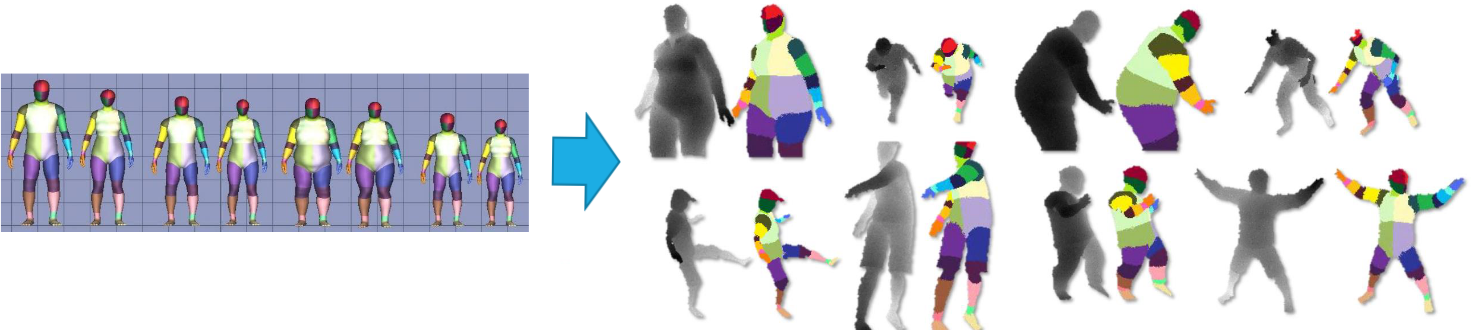
\includegraphics[width=0.75\linewidth]{./img/motion_data.png}
        \end{figure}

    \item[Depth comparison features] \marginnote{Depth comparison features}
        Given a depth image $D$ and the offsets $\theta = (\Delta p, \Delta n)$, each pixel $x$ of $D$ produces a feature as follows:
        \[ f(x; D, (\Delta p, \Delta n)) = D\left[ x + \frac{\Delta p}{D[x]} \right] - D\left[ x + \frac{\Delta n}{D[x]} \right] \]
        In other words, each $x$ is described by the difference in depth between two points offset from $x$. The depth at background pixels is a large positive number.

        \begin{remark}
            As real-time processing is required, this approach allows to quickly compute features to discriminate parts of the body. However, it does not always produce a correct response.
        \end{remark}

        \begin{figure}[H]
            \centering
            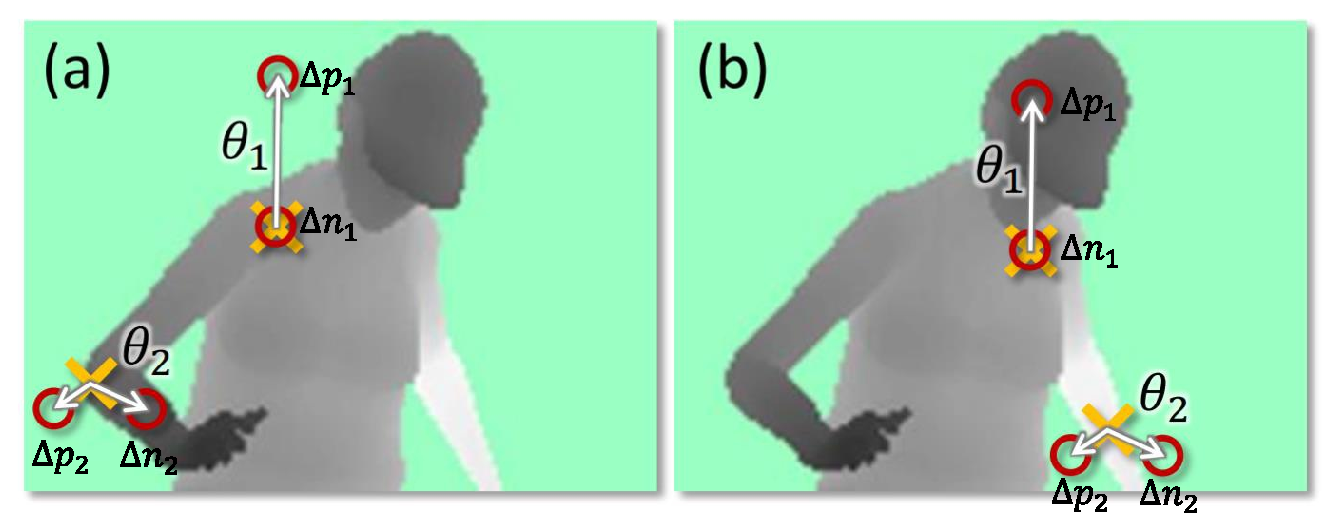
\includegraphics[width=0.6\linewidth]{./img/_depth_comparison_features.pdf}
            \caption{Examples of feature computation}
        \end{figure}

        \begin{description}
            \item[Depth-invariant offsets]
                The denominator ($D[x]$) applied to the offsets allows obtaining depth-invariant offsets.

                Consider two objects at different depths. The focal length of the camera is $f$ and the world offset we want to apply is $o_w$. By changing depth $d$, the offset in the image plane $o_{di}$ changes due to the perspective projection rules. Therefore, to obtain the offset in the image place, we have that:
                \[ o_{di} : f = o_w : d \,\Rightarrow\, o_{di} = \frac{o_w f}{d} = \frac{\Delta p}{d} \]

                \begin{figure}[H]
                    \centering
                    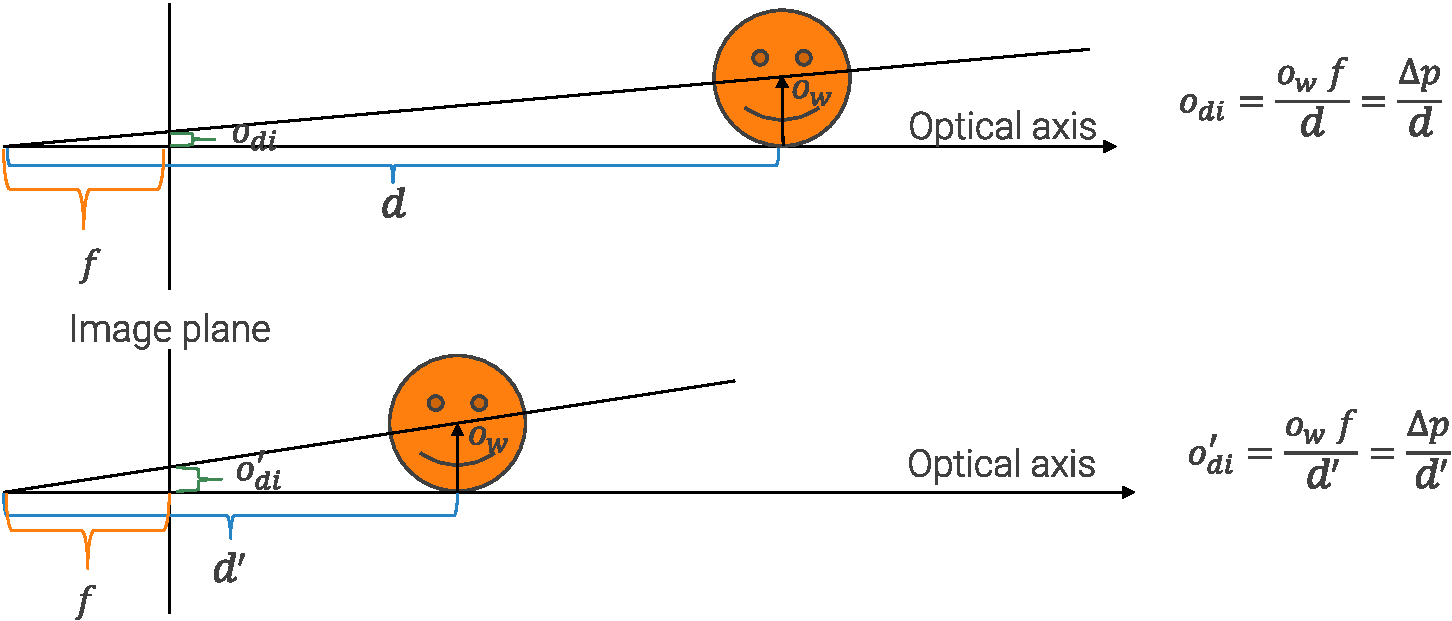
\includegraphics[width=0.6\linewidth]{./img/_depth_invariant_offset.pdf}
                \end{figure}
        \end{description}

    \item[Decision tree] \marginnote{Decision tree}
        Depth comparison features are used to train decision trees.

        \begin{remark}
            Decision trees are unstable robust classifiers. They are able to achieve good performance but significantly change in structure if the training data is slightly perturbed (i.e., high variance).
        \end{remark}

        \begin{description}
            \item[Random forest] \marginnote{Random forest}
                Ensemble of $N$ decision trees that aims to reduce variance by averaging their predictions.

                \begin{remark}
                    For a random forest to be effective, its decision trees should be uncorrelated so that when averaging, the average of their errors tend to $0$.
                \end{remark}

                \begin{description}
                    \item[Bootstrap aggregating (bagging)] \marginnote{Bootstrap aggregating (bagging)}
                        Train each decision tree using a replica of the training set obtained by sampling with replacement.

                        \begin{figure}[H]
                            \raggedleft
                            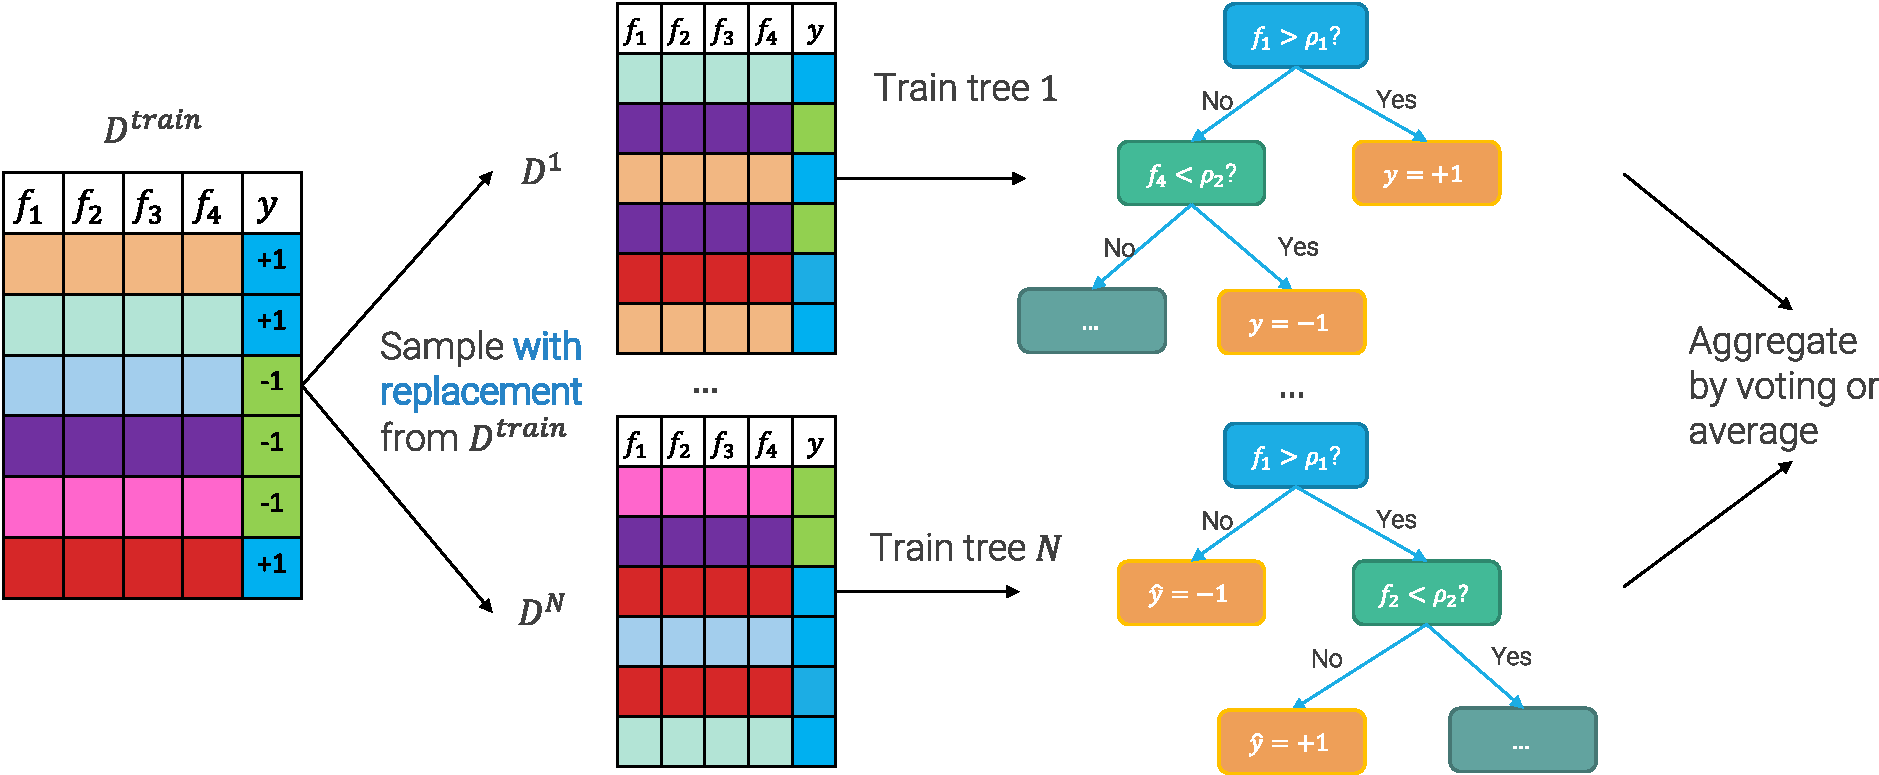
\includegraphics[width=0.7\linewidth]{./img/_random_forest_bagging.pdf}
                        \end{figure}

                    \item[Random splitting] \marginnote{Random splitting}
                        Even though bagging reduces variance, if there is a subset of particularly predictive features, the resulting trees will be correlated. 

                        To avoid this, in a random forest, tree splitting is done on a different random subset of features each time.

                        \begin{figure}[H]
                            \raggedleft
                            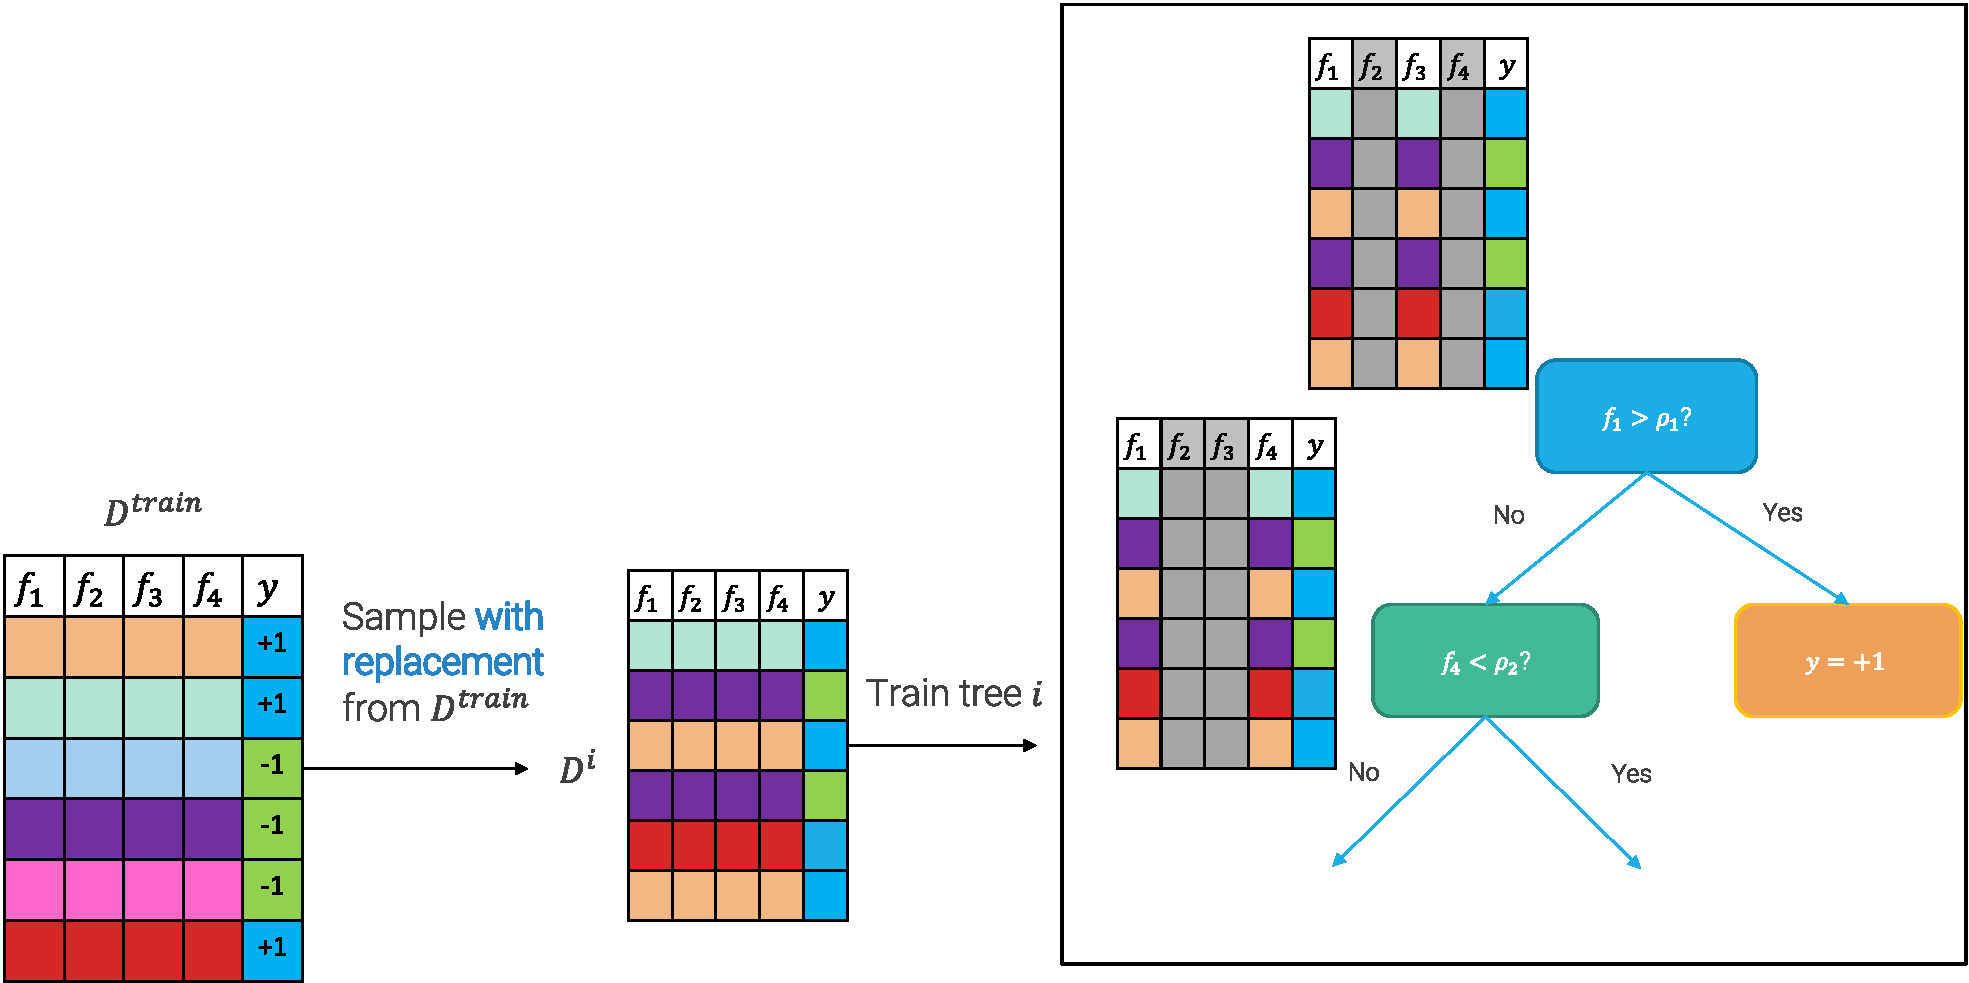
\includegraphics[width=0.7\linewidth]{./img/_random_forest_random_splitting.pdf}
                        \end{figure}
                \end{description}

                \begin{remark}
                    Random forests are:
                    \begin{itemize}
                        \item Fast and parallelizable in both training and inference.
                        \item Robust to hyperparameters change.
                        \item Interpretable.
                    \end{itemize}
                \end{remark}
        \end{description}
\end{description}